% Contributors: Alexandre Lamy, Trung Vu
\section{The DBSCAN algorithm}
  DBSCAN stands for \textbf{D}ensity \textbf{B}ased \textbf{S}patial
  \textbf{C}lustering  for \textbf{A}pplication with \textbf{N}oise. This
  algorithm was proposed by Ester, Kriegel, Sander, and Xu in 1996. In 2014,
  the original paper won the Test of Time Award from \textit{Knowledge Discovering and Data Mining},
  the top journal in data mining.
  \subsection{Basic idea}
  There are two parameters to the DBSCAN algorithm: $\epsilon$ and $m$, which
  controls which point qualifies as being in a dense region. Based on $\epsilon$
  and $m$, we classify the data points of into 3 kind of data points:

  \begin{enumerate}
  \item Core points: These are the points which are considered to be in a
  dense region, where dense is defined precisely as follows: given a point $x$,
  consider the $\epsilon$-ball around it, and if the $\epsilon$-ball has
  at least $m$ data points around it, then we consider it a core point. Formally,
  if we denote the set of core points as $C$, then $C=\{x \in X \ | \ X \cap B(x,\epsilon)\geq m\}$.
  \item Border points: These are points that do not satisfy the $\epsilon$-ball
  density condition for core points, but is within $\epsilon$ of a core point.
  Note that if a border point is within $\epsilon$ of more than 1 data point
  then we break ties arbitrarily. Note that this implies that DBSCAN is sensitive
  to the order of the input data. These points are consider to be the "boundary"
  of our dense region: they are "buffer zones" for which the density of our regions
  taper off before the become low-density.
  \item Noise points: These are points that neither satisfy the condition for
  core points or border points. Since they are so far away from the core points,
  they should be considered noisy data points sampled from low-density regions.
  \end{enumerate}

  The intuition here is that dense regions (to be precise, $m$ data points within
  an $\epsilon$ ball) that are close enough (to be precise, within $\epsilon$ of each other),
  should be consider as part of a bigger dense region. Thus we connect core
  points if they are within $\epsilon$ of each other. To find connected regions,
  we simply run connected components on the graphs constructed from the core
  points, where we put edges between the core points in the graph if they are
  close enough (again, this means they are within $\epsilon$ of each other).

  To make this more vivid, consider the figure below. The red point is a core point:
  it has high-density in the $\epsilon$-ball around it. The yellow point is a border
  point: it has low-density in the region around it but is within $\epsilon$ of
  a core point. The gray point is a noise point, since it $\epsilon$-ball
  contains no points other than itself, and it is far away from the two high-density
  regions, which are marked with red boundaries.

  \begin{figure}[h]
  \centering
  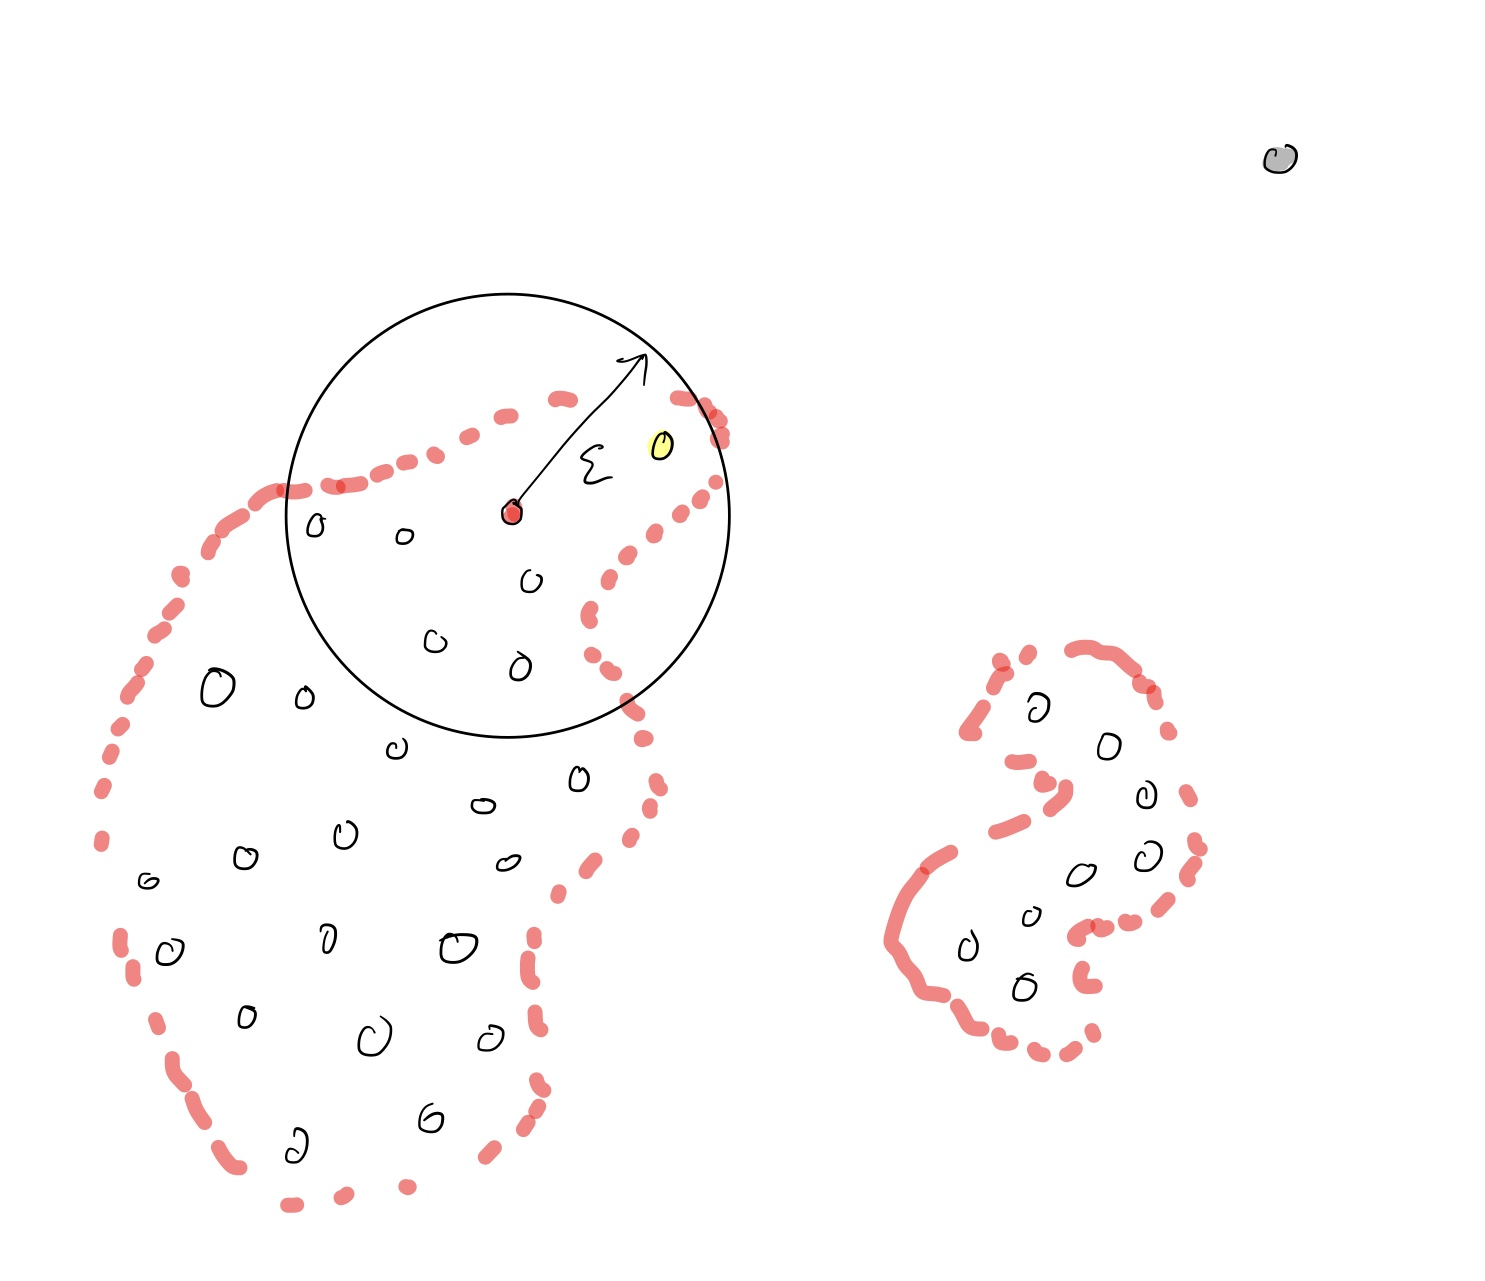
\includegraphics[width=.7\linewidth]{chapter_2/files/dbscan.jpg}
  \caption{Visualization of DBSCAN}
  \end{figure}

  We can also see that if we take our core points as our vertices, put an edge between
  the core points that are close to each other and run connected components on
  the graph, then we will get precisely the two partitions above.

  \subsection{The algorithm}

  We include a formal definition of the algorithm:

  \begin{enumerate}
  \item Let $C=\{x \in X \ | \ X \cap B(x, \epsilon) \geq m\}$.
  \item Construct the graph $G=(V,E)$, with $V=C$, $E=\{(i,j) \ | \ ||x_i-x_j|| \leq \epsilon\}$.
  \item Run connected components on $G$. The clusters are the connected components
  \item Let $B=\{x \in X \ | \ x \notin C, \exists c \in C, ||x-c|| \leq \epsilon\}$.
  For each $b \in B$, assign $b$ to the connected component of any arbitrary $c$
  that is within $\epsilon$ of $b$.
  \item Ignore the rest of the points, which we consider noise points.

  \end{enumerate}

  \subsection{Pros and Cons}
  Cons:
  \begin{itemize}
    \item DBSCAN is very sensitive to the parameter settings. In other words, the algorithm could return excellent clusters for some value of $\epsilon$ and $m$
    and very bad ones for a different, but close, setting of $\epsilon$ and $m$. To avoid this drawback one can try many different values for the parameters and/or use
    some kind of parameter search (also called hyperparameter optimization) method.
    \item Different clusters could have different densities. This would mean that there is no single global setting of $\epsilon$ and $m$ which will work for all clusters.
    There is a modification of DBSCAN called OPTICS which partially solves this problem. The core idea of this modification is use very tight parameters to find a very
    dense cluster, remove that cluster from the data, relax the parameters, and repeat.
    \item DBSCAN does not work in high dimensions. This is the main drawback of DBSCAN. The issue is that in high dimensions, in practice, almost all points are
    at almost identical distances from each other. As a result, depending on the parameters, either all points are ``close'' to each other and we get one big
    cluster, or all points are ``far'' from each other and we get no clusters.
  \end{itemize}
  Pros:
  \begin{itemize}
    \item The number of clusters $k$ does not need to be specified.
    \item DBSCAN can find clusters of arbitrary shape, it makes no assumptions on the shape of the clusters (whereas centroid based methods assume that the clusters are convex, as discussed above).
    \item It has bounded runtime and runs relatively fast in practice.
  \end{itemize}

  \subsection{An example}
  Foursquare is a company with an app that, among other things, allows users to ``check-in'' by providing information on where they are. This is stored along with their current GPS position.
  Then a modification of the DBSCAN algorithm is used to estimate the ``boundaries'' between the different locations that users checked in too. This allows Foursquare to predict the establishment that
  their users are in simply from their GPS data. Interestingly, they use a random forest to predict the parameters of DBSCAN. There is more information on Foursquare and their use of
  DBSCAN available on the web, as well as many more examples of real life uses of DBSCAN.
